\documentclass[Arkitektur/System_main.tex]{subfiles}
\begin{document}
\subsubsection{Fra User stories til arkitektur}
User Story Distribution Diagrammet viser User Stories sammenhæng med arkitekturen. De andre views tager udgangspunkt i distributionerne. 
\begin{figure}[H]
    \centering
    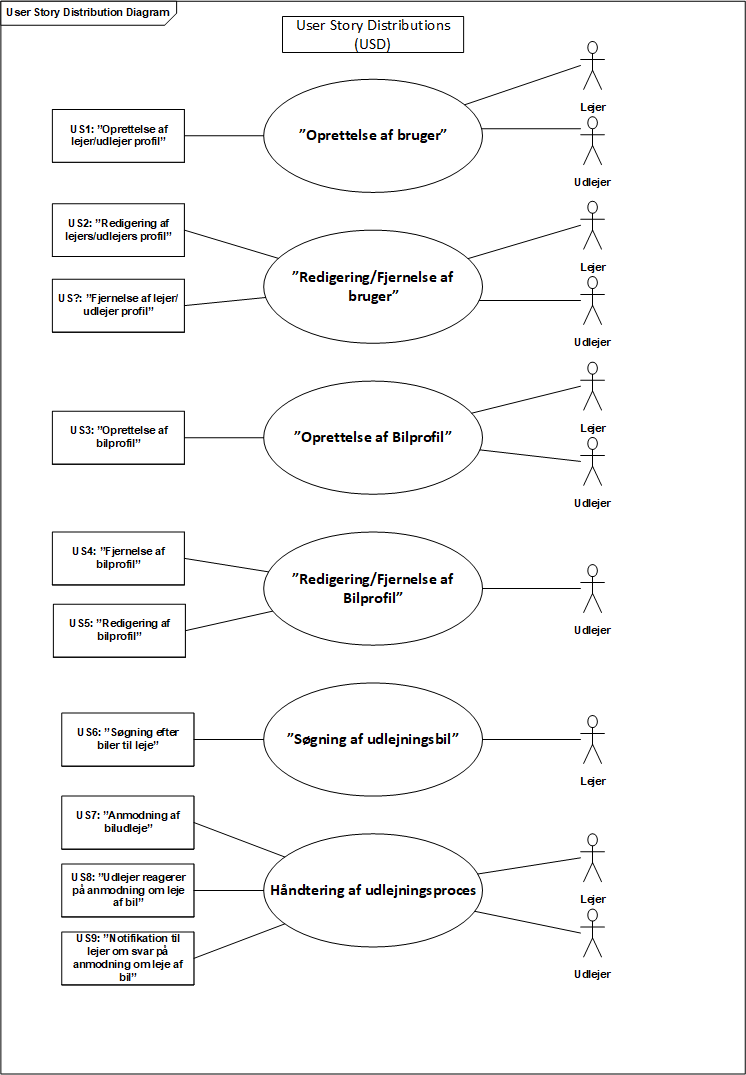
\includegraphics[width=0.90\textwidth]{Kravspecifikation/Funktionelle_krav/UserStories/graphics/USDD.png}
    \caption{User Story Distribution Diagram (USDD)}
    \label{fig:USDD}
\end{figure}
Disse User Stories er designet ud fra domænet, som implicit blev introduceret i Problemformulering og Kravspecifikationen. For at konceptualiserer domænet og beskrive dets adfærd og data, er der lavet en domænemodel. Domænemodellem angiver systemets eksterne og interne aktører/roller, som interagerer med softwarekomponenter og data. Domænemodellen ses nedenfor.
\begin{figure}[H]
    \centering
    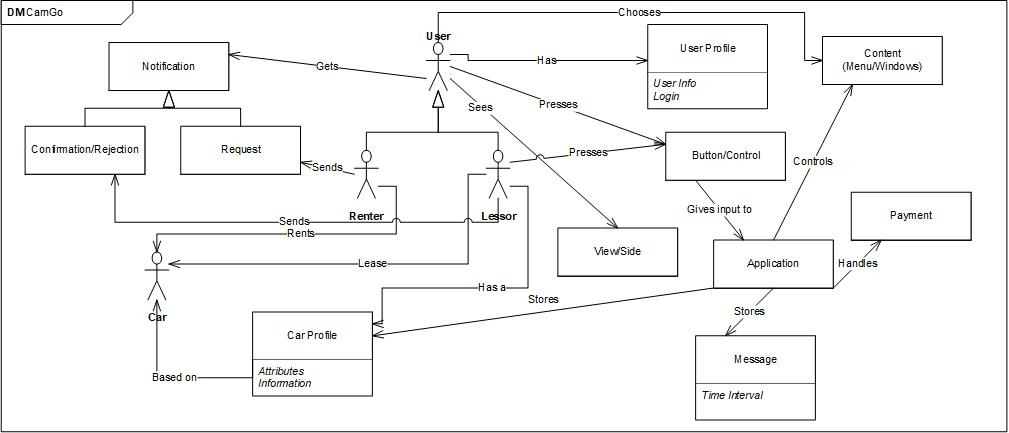
\includegraphics[width=1\textwidth]{Arkitektur/Softwarearkitektur/UserStoryArchitecture/graphics/DomainModel.jpg}
    \caption{Domænemodel af CarnGo-systemet.}
    \label{fig:domain}
\end{figure}
I domænemodellen introduceres alle rollerne i systemet, og hvilke rettigheder og muligheder de har i forhold til interaktionen med systemet og dets data. Kasserne skal ses som softwarekomponenter eller koncepter for systemet. Aktørerne er de roller brugeren kan have i systemet - de er en bruger, indtil de registreres i systemet; enten som lejer eller udlejer. \\\\
Nu hvor systemets koncepter er illustreret, er det muligt at beskrive dets arkitektur. De næste afsnit vil gennemgå systemets arkitektur, grænseflade og adfærd. 
\end{document}